\documentclass{fizykalab}

% Ustawienia do tabelki

\wydzial{WI}
\autorjeden{Piotr Karamon}
\autordwa{Hubert Kasprzycki}
\rok{2}
\grupa{12}
\zespol{5}
\temat{Wahadło proste}
\nrcwiczenia{}
\datawykonania{03.10.2023}
\dataoddaniajeden{10.10.2023}
\zwrotdopoprawy{}
\dataoddaniadwa{}
\datazaliczenia{}



\usepackage{amsmath}
\usepackage{parskip}


\newcolumntype{L}[1]{>{\raggedright\let\newline\\\arraybackslash\hspace{0pt}}m{#1}}
\newcolumntype{C}[1]{>{\centering\let\newline\\\arraybackslash\hspace{0pt}}m{#1}}
\newcolumntype{R}[1]{>{\raggedleft\let\newline\\\arraybackslash\hspace{0pt}}m{#1}}

\usepackage[left=1.75cm, right=2cm, top=3cm]{geometry}
\usepackage[labelfont=bf]{caption}

\usepackage{natbib}
\usepackage{url}
\begin{filecontents*}{test.bib}
@misc{Wahadło,
  title = {M101. Przemiany energii w ruchu wahadła},
  author = {},
  note  =  {\url{https://ppef.amu.edu.pl/images/materialy-dydaktyczne/filami/pl/M102-Wahadlo.pdf}},
  note = {Odwiedzona: 9-10-2023},
}

\end{filecontents*}

\begin{document}

\newcommand{\mss}{\ensuremath{\frac{\text{m}}{\text{s}^2}}}


\maketitle

\section{Cel ćwiczenia}
\begin{itemize}
    \item Zaznajomienie się z typowymi metodami opracowania danych pomiarowych w laboratoriach fizycznych 
    \item Zapoznanie się z ruchem drgającym na przykładzie drgań wahadła prostego
    \item Wyznaczenia przyśpieszenia ziemskiego
\end{itemize}


\section{Aparatura pomiarowa}
\begin{itemize}
    \item Stoper w telefonie o dokładności $0.01\text{s}$
    \item Przymiar milimetrowy o dokładności $1\text{mm}$
\end{itemize}


\section{Wstęp teoretyczny}
\begin{figure}[H]
    \centering
    \includegraphics[width=0.5\linewidth]{wahadło.png}
    \caption{\cite{Wahadło} Wahadło proste jest obiektem który składa się z ciała o masie punktowej równej $m$,
             które jest zawieszone na nieważkiej, nierozciągliwej nici o długości $l$.
             Nić ma stały punkt przyłożenia. Na ciało działa siła grawitacji.
             Składowa $\vec{F}^{\bot}_G$ powoduje ruch wahadłowy.
             }
    \label{fig:enter-label}
\end{figure}

W pracowni cienką nierozciągliwą nić nawinięto na wysoko położony walec. Następnie na dole nici zawieszono 
jednorodny walec. Uzyskany w ten sposób obiekt fizyczny ma zbliżone właściwości do teoretycznego wahadła prostego.

Okres drgań wahadła prostego dla wychyleń o małych kątach wyraża się wzorem

\begin{equation}
    \label{eq_period}
    T = 2\pi\sqrt{\frac{l}{g}}
\end{equation}

Z tego równania można wyznaczyć przyśpieszenie grawitacyjne $g$.

\begin{equation}
    \label{eq_g}
    g = \frac{4\pi^2l}{T^2}
\end{equation}

\section{Przebieg doświadczenia}

\subsection{Sposób pierwszy}

Mierzymy długość wahadła, a następnie mierzymy czas dziesięciu pełnych drgań wahadła.
\begin{table}[H]
    \centering
    \begin{tabular}{|C{3cm}|C{3cm} | C{3cm}|}
        \hline
        $l$ [mm] & Czas \textit{t} dla 10 okresów [s]& Okres $T = t/10$ [s]\\ [0.5ex] 
        \hline
        \hline
        357 & 12.03 & 1.203\\ \hline
    \end{tabular}
\end{table}

Przyjmujemy, że w związku z błędami ludzkimi niepewności pomiaru długości wahadła $l$ wynosi:
\begin{equation}
    u(l) = 2\text{mm}
\end{equation}

Natomiast niepewność pomiaru czasu odczytanego ze stopera, wynosi:
\begin{equation}
    u(t) = 0.3\text{s}
\end{equation}


Skoro $t=10T$ $\implies$ $u(T) = u(10T)/10 = 0.03\text{s}$.

Aby wyliczyć niepewność pomiaru $g$ stosujemy prawo przenoszenia niepewności, ponieważ
zmierzony okres oraz długość nie są skorelowane a ich niepewności są dużo mniejsze od wartości.

\begin{equation} 
\label{eq_ug}
u(g) = \sqrt{  
    {\left( \frac{\partial g}{\partial l}u(l) \right)}^2 + 
    {\left(\ \frac{\partial g}{\partial T}u(T) \right)}^2 
}   = \sqrt{  
    {\left(  \frac{4\pi^2}{T^2}u(l) \right)}^2 + 
    {\left(  \frac{-8\pi^2l}{T^3}u(T) \right)}^2
} 
\end{equation}

Podstawiając wartości do równań (\ref{eq_g}) oraz (\ref{eq_ug}) otrzymujemy:
\begin{align*}
    u(g) &= 0.49 \mss \\
    g &= 9.74 \mss
\end{align*}


\subsection{Sposób drugi}
Mierzymy długość wahadła $l$, a następnie dziesięć razy mierzymy czas dziesięciu pełnych drgań wahadła.
Długość wahadła nie uległa zmianie i jak w sposobie pierwszym $l = 357 \text{mm}$ tak samo jak $u(l) = 2mm$.

\begin{table}[H]
    \centering
    
    \begin{tabular}{|C{3cm}|C{3cm}|C{3cm}|}
        \hline
        Lp. & Czas \textit{t} dla 10 okresów [s]& Okres $T = t/10$ [s]\\ [0.5ex] 
        \hline
        \hline
        
        1  & 12.03 & 1.203\\ \hline
        2  & 11.95 & 1.195\\ \hline
        3  & 11.99 & 1.199\\ \hline
        4  & 11.92 & 1.192\\ \hline
        5  & 11.98 & 1.198\\ \hline
        6  & 11.81 & 1.181\\ \hline
        7  & 11.81 & 1.181\\ \hline
        8  & 11.98 & 1.198\\ \hline
        9  & 11.48 & 1.148\\ \hline
        10 & 11.87 & 1.187\\ \hline
    \end{tabular}
    \label{tab:my_label}
\end{table}


Najpierw liczymy średni okres.

\begin{equation}
    \overline{T} = \frac{\sum_{i=1}^{10}{T_i}}{10} = 1.1882 \text{s}
\end{equation}

Aby obliczyć niepewność pomiaru okresu używamy estymatora odchylenia standardowego średniej

\begin{equation}
u(\overline{T}) = \sqrt{ \frac{ \sum_{i=1}^{10}{(T_i - \overline{T})}^2  }{n(n-1)} }
\end{equation}

Wyliczamy niepewność $\overline{T}$ a następnie podstawiamy do równań (\ref{eq_g}) oraz (\ref{eq_ug})
pamiętając, że $u(\overline{T})$ wstawiamy w miejsce $u(T)$ a $\overline{T}$ w miejsce $T$.

\begin{align*}
    u(\overline{T}) &= 0.0051 \text{s} \\
    u(g) &=  \sqrt{  
    {\left(  \frac{4\pi^2}{\overline{T}^2}u(l) \right)}^2 + 
    {\left(  \frac{-8\pi^2l}{\overline{T}^3}u(\overline{T}) \right)}^2} = 0.11 \mss \\
    g &= \frac{4\pi^2l}{\overline{T}^2} = 9.98 \mss \\
\end{align*}

Teraz możemy obliczyć niepewność rozszerzoną, przyjmując $k=2$
\begin{equation*}
    U(g) = ku(g) = 2 \cdot 0.11 \mss = 0.22 \mss
\end{equation*}

Z tego wynika, że
\begin{equation*}
    g = 9.98 \mss \pm 0.22 \mss
\end{equation*}

Wartość tabelaryczna przyspieszenia ziemskiego dla Krakowa wynosi $g = 9.81 \mss$ 
a więc otrzymana przez nas wartość jest z nią zgodna.

\subsection{Sposób trzeci}
Dokonujemy sześciu pomiarów dla różnych długości wahadła $l$. Za każdym razem mierzymy czas dziesięciu pełnych drgań wahadła.

\begin{table}[H]
    \centering
    
    \begin{tabular}{|C{2cm}|C{2cm}|C{2cm}|C{2cm}|}
        \hline
        $l$ [mm] & Czas \textit{t} dla 10 okresów [s]& Okres $T = t/10$ [s] & $T^2$ [$\text{s}^2$] \\ [0.5ex] 
        
        \hline
        \hline
        
        97   & 6.14  & 0.614 & 0.376996 \\   \hline
        144  & 7.45  & 0.745 & 0.555025 \\   \hline
        190  & 8.62  & 0.862 & 0.743044 \\   \hline
        237  & 9.50  & 0.950 & 0.902500 \\   \hline
        323  & 11.20 & 1.120 & 1.254400 \\   \hline
        400  & 12.27 & 1.227 & 1.505529\\   \hline
    \end{tabular}
\end{table}

Z równania (\ref{eq_period})

\begin{align*}
    \label{eq_period_sqr}
    T^2 &= \frac{4\pi^2l}{g}\\
    T^2 &= al \qquad \text{gdzie  } a = \frac{4\pi^2}{g} = \text{const}
\end{align*}

Z tego wynika, że zależność kwadratu okresu jest liniowa względem długości wahadła.

\begin{figure}[H]
    \centering
    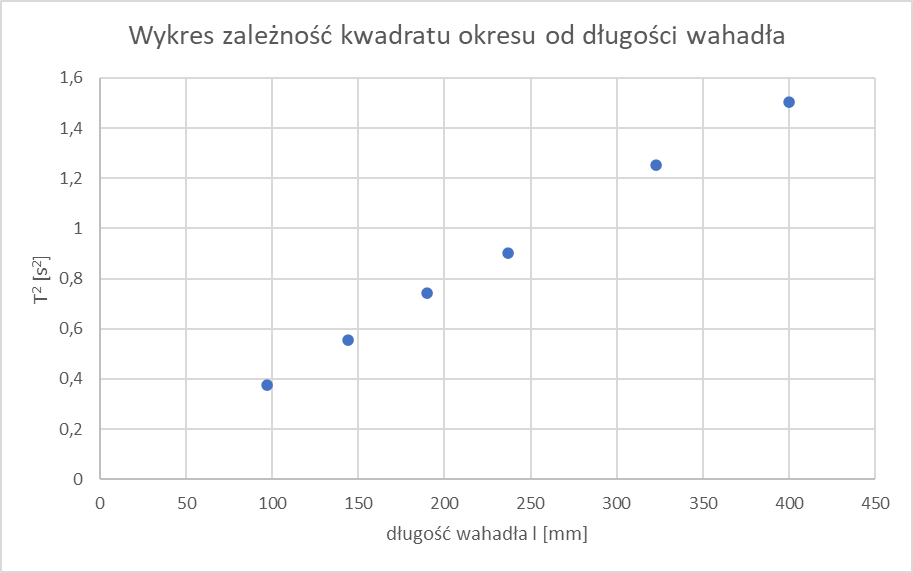
\includegraphics[width=0.75\linewidth]{wykres-1.png}
    \label{fig:enter-label}
\end{figure}

\begin{figure}[H]
    \centering
    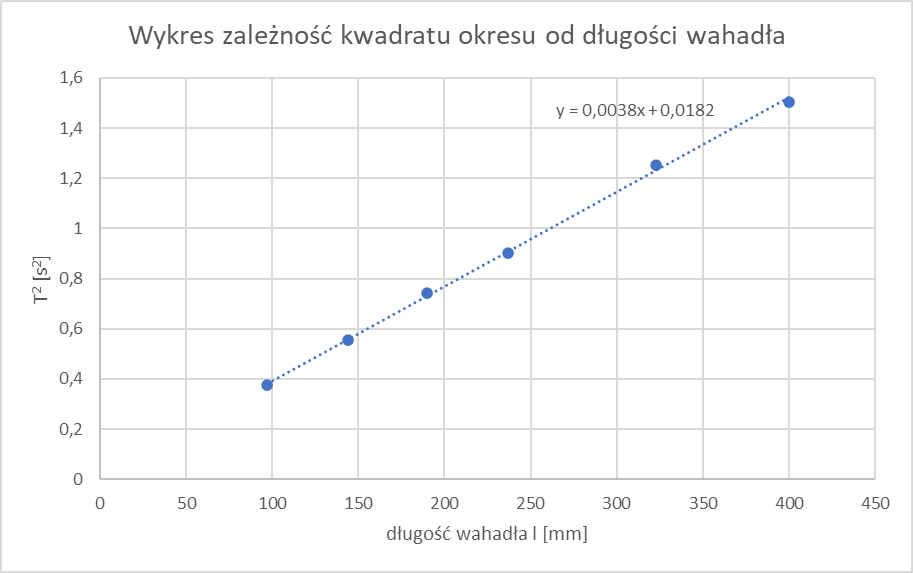
\includegraphics[width=0.75\linewidth]{wykres-2.png}
    \label{fig:enter-label}
\end{figure}


Otrzymujemy prostą o równaniu: 

\begin{equation*}
    y = 0.0038x + 0.0182
\end{equation*}

Zatem

\begin{equation*}
    a = 3.8\frac{s^2}{m}
\end{equation*}

Aby obliczyć niepewność $u(g)$ stosujemy prawo przenoszenia niepewności.
Tym razem $g$ jest funkcją tylko jednej zmiennej $a$. Program liczący liniową regresję również 
obliczył niepewność $a$ która wynosi $u(a) = 0.061 \frac{\text{s}^2} {\text{m}}$


\begin{equation*}
    u(g) = \sqrt{\left(\frac{\partial g}{\partial a}u(a)\right)^2} = \left|\frac{-4\pi^2}{a^2}u(a)\right| = 0.17 \mss
\end{equation*}


Wartość g obliczamy korzystając ze wzoru $a=\frac{4\pi^2}{g}$ odpowiednio go przekształcając:
\begin{equation*}
    g = \frac{4\pi^2}{a} = 10,39 \mss
\end{equation*}

\section{Wnioski}
W wyniku przeprowadzenia trzech różnych podejść otrzymaliśmy wartości $g$ które
w różnym stopniu różnią się od wartości tabelarycznej. Sposoby różniły się znacząco
stopniem skomplikowania. Od pierwszego, który można wykonać używając kartki
papieru i kalkulatora prostego, do trzeciego w którym korzystaliśmy już z
arkusza kalkulacyjnego i liniowej regresji. 

Wraz ze stopniem zaawansowania
metody udawało nam się uzyskiwać coraz mniejszą niepewność $u(g)$. Zdziwił nas
natomiast fakt, iż wartość $g$ w sposobie ostatnim najbardziej odbiega od
wartości tabelarycznej. Możliwym jest, że wynik ten tak diametralnie odbiega od
wartości tabelarycznej ponieważ wymagał wielokrotnego mierzenia długości
wahadła. Pomiar długości był wykonywany przez wiele osób, pewnie z różniącą się 
dbałością. Był on jednocześnie o wiele trudniejszy od pomiaru okresu w którym
wystarczyła odrobina refleksu. Mierząc długość należało być bardzo ostrożnym 
jeżeli chodzi o wyznaczenie punktu przyłożenia oraz środka masy cylindra.

Wyniki wyznaczone w trzech sposobach różnią się między sobą oraz są inne od
wartości tabelarycznej, istnieje ku temu kilka powodów:
\begin{itemize}
    \item Błędy ze strony ludzkiej - złe przyłożenie przymiaru 
    milimetrowego do środka cylindra i punktu przyłożenia nici.
    Zbyt wolna reakcja przy mierzeniu czasu.
    \item Niedokładność przyrządów pomiarowych.
    \item Możliwe, że wychylanie masy o za duży kąt przy którym wzór na okres drgań wahadła
          staje się już wyraźnie nieprecyzyjny. 
    \item Założenie, że mamy do czynienia z wahadłem prostym a nie fizycznym.
    \item Ciężarek był walcem, możliwe że przy użyciu kulki otrzymalibyśmy lepsze wyniki.
\end{itemize}



\renewcommand{\refname}{Bibliografia}
\bibliographystyle{abbrv}
\bibliography{test}


\end{document}
 
 
 

 


